\chapter{Anforderungstabellen nach ISO 9241-110}
\label{Add:ISO-Tabellen}

\begin{table}[H]
    \centering
    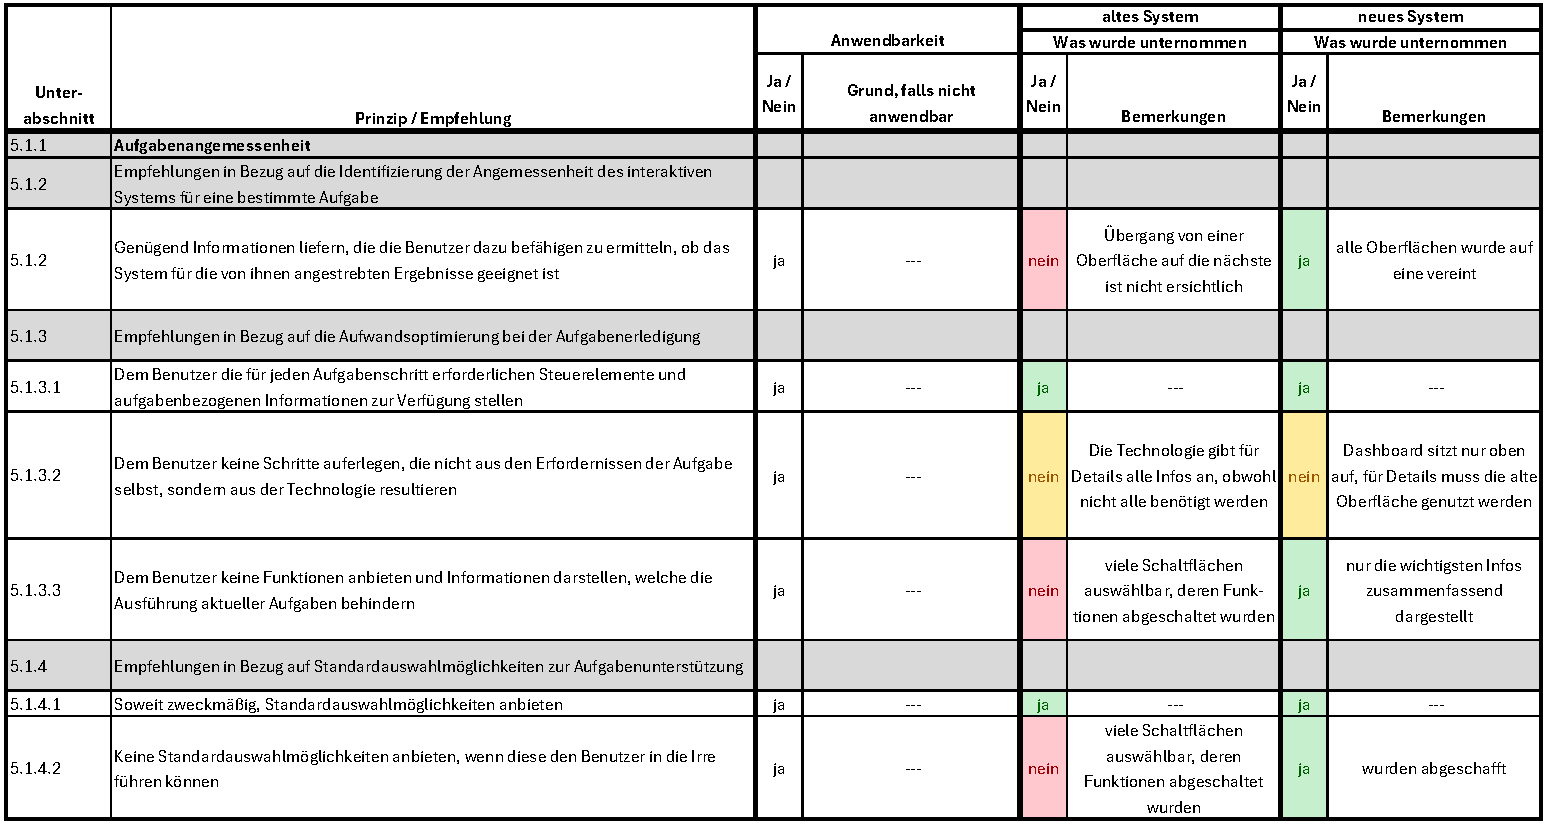
\includegraphics[width=0.8\textheight, angle=90]{Anhänge/02_ISO-Tabellen/01_Aufgabenangemessenheit.pdf}
    \caption{Zustands- und Anforderungsanalyse sowie Vergleich des alten und neuen Systems nach \cite{DIN_EN_ISO_9241-110} (1/7 Aufgabenangemessenheit)} % S. 36-41
    \label{tab:Anforderungskatalog_ISO_alt_neu_1}
\end{table}

\begin{table}[H]
    \centering
    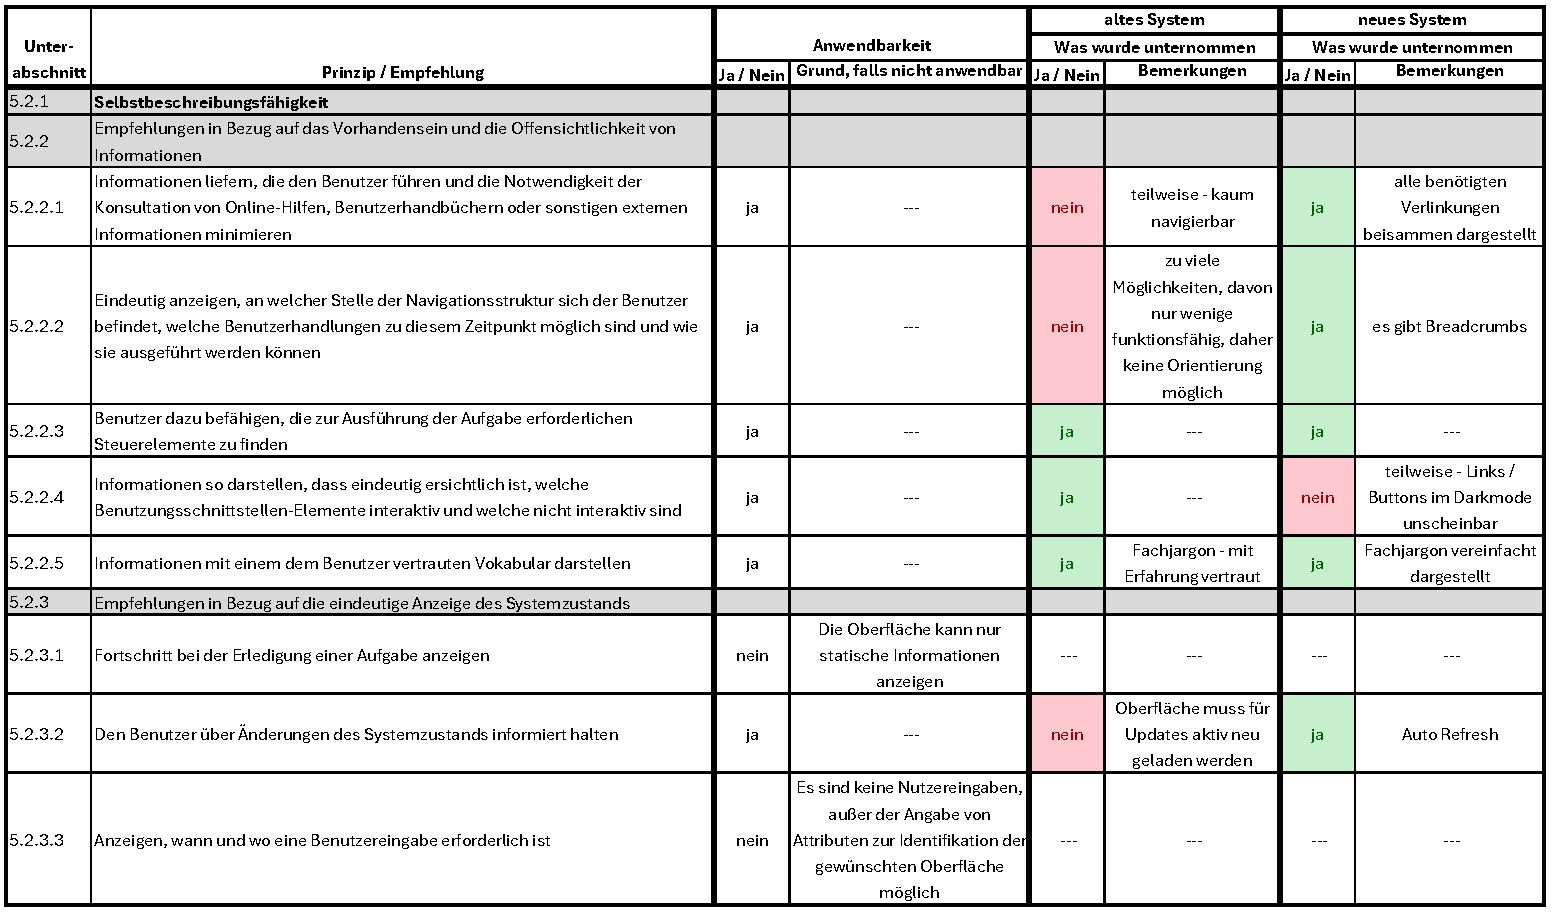
\includegraphics[width=0.95\textheight, angle=90]{Anhänge/02_ISO-Tabellen/02_Selbstbeschreibungsfaehigkeit.pdf}
    \caption{Zustands- und Anforderungsanalyse sowie Vergleich des alten und neuen Systems nach \cite{DIN_EN_ISO_9241-110} (2/7 Selbstbeschreibungsfähigkeit)}
    \label{tab:Anforderungskatalog_ISO_alt_neu_2}
\end{table}

\begin{table}[H]
    \centering
    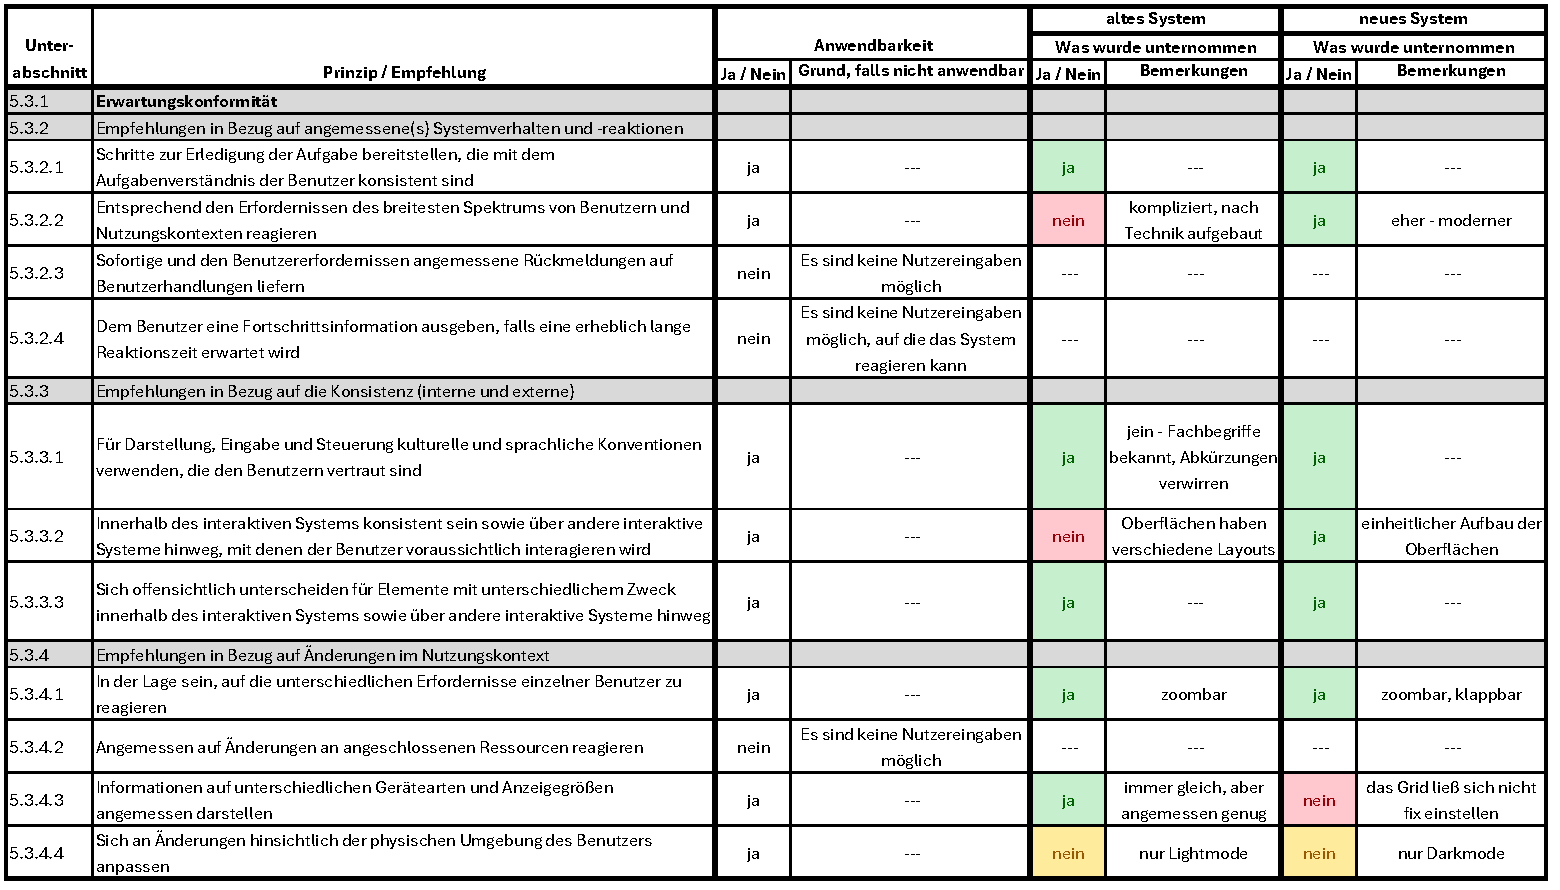
\includegraphics[width=0.95\textheight, angle=90]{Anhänge/02_ISO-Tabellen/03_Erwartungskonformitaet.pdf}
    \caption{Zustands- und Anforderungsanalyse sowie Vergleich des alten und neuen Systems nach \cite{DIN_EN_ISO_9241-110} (3/7 Erwartungskonformität)}
    \label{tab:Anforderungskatalog_ISO_alt_neu_3}
\end{table}

\begin{table}[H]
    \centering
    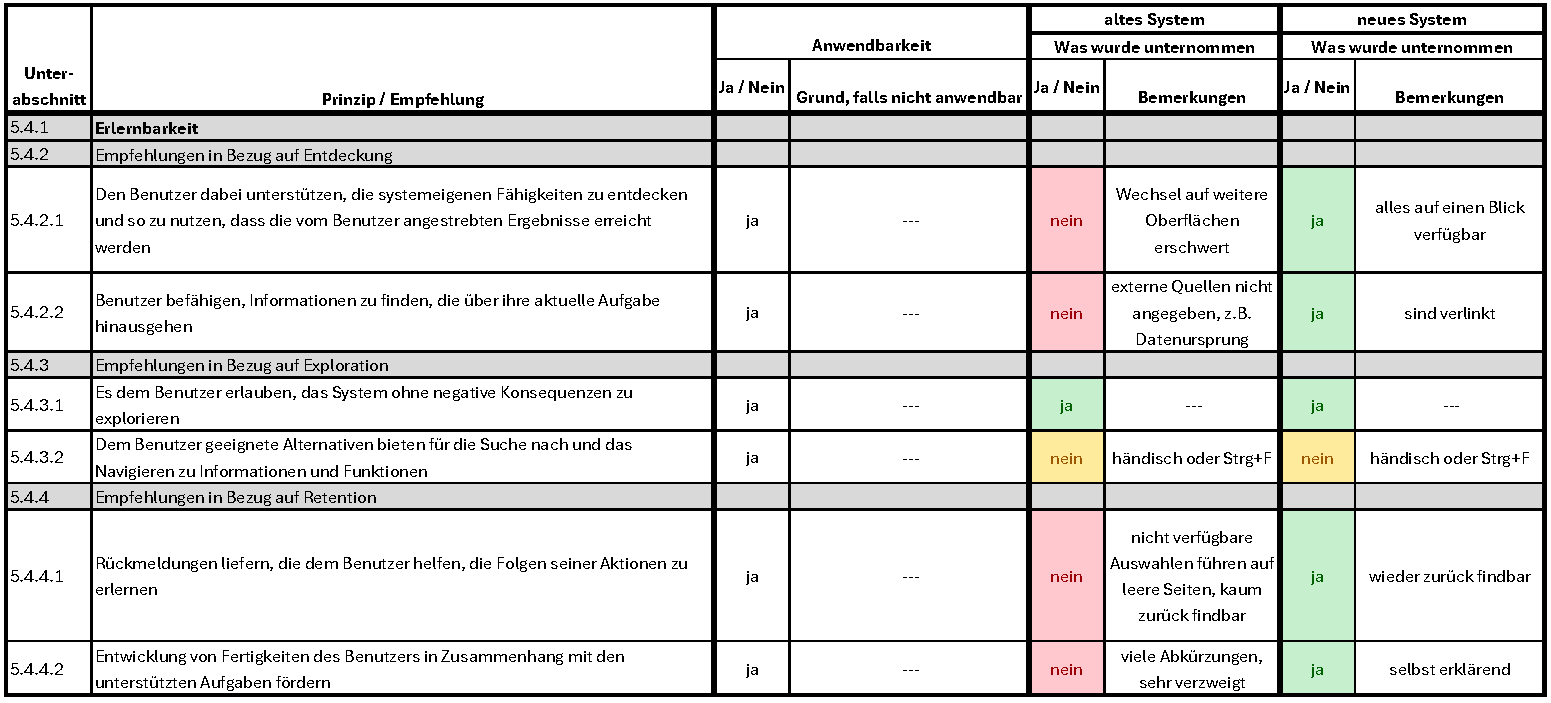
\includegraphics[width=0.95\textheight, angle=90]{Anhänge/02_ISO-Tabellen/04_Erlernbarkeit.pdf}
    \caption{Zustands- und Anforderungsanalyse sowie Vergleich des alten und neuen Systems nach \cite{DIN_EN_ISO_9241-110} (4/7 Erlernbarkeit)}
    \label{tab:Anforderungskatalog_ISO_alt_neu_4}
\end{table}

\begin{table}[H]
    \centering
    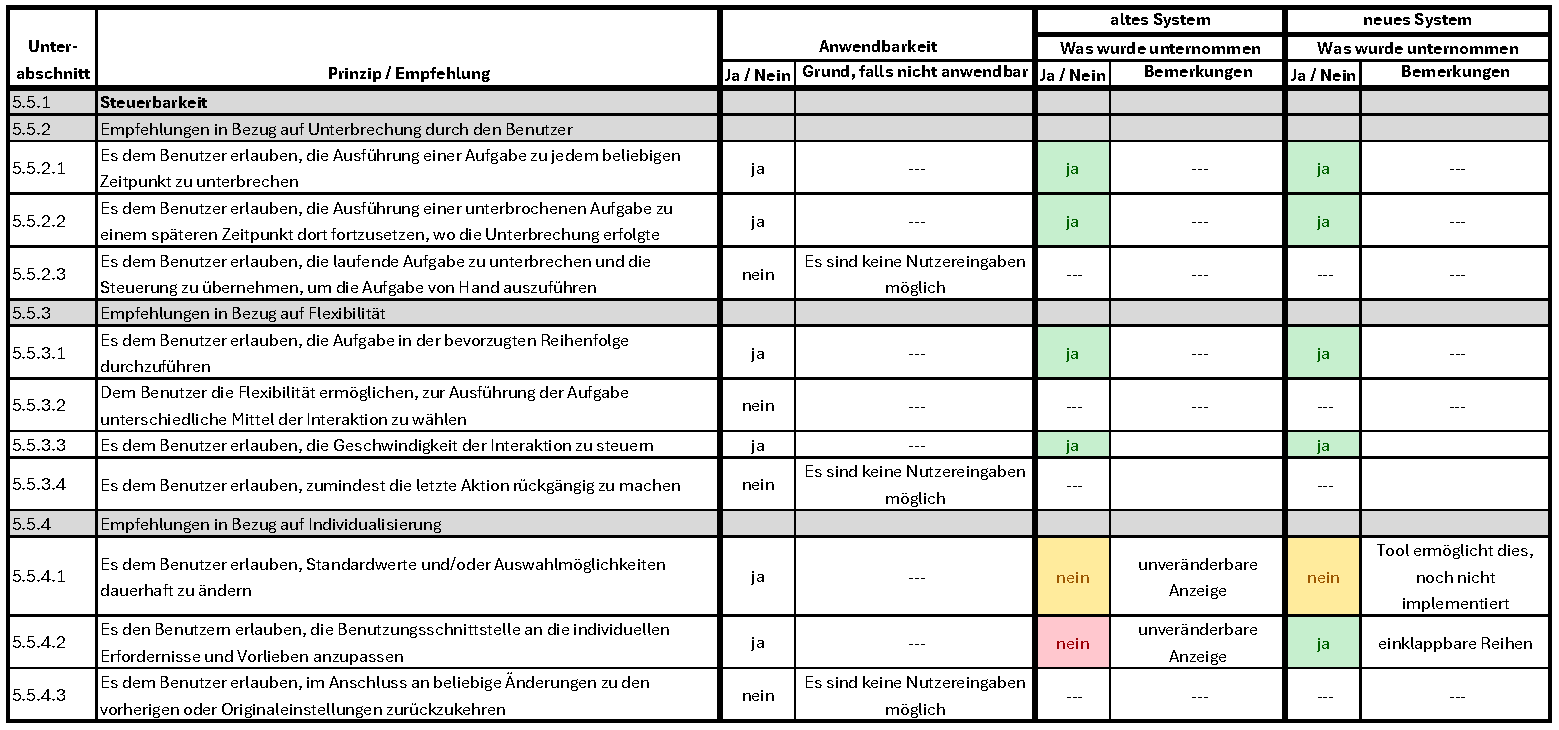
\includegraphics[width=0.95\textheight, angle=90]{Anhänge/02_ISO-Tabellen/05_Steuerbarkeit.pdf}
    \caption{Zustands- und Anforderungsanalyse sowie Vergleich des alten und neuen Systems nach \cite{DIN_EN_ISO_9241-110} (5/7 Steuerbarkeit)}
    \label{tab:Anforderungskatalog_ISO_alt_neu_5}
\end{table}

\begin{table}[H]
    \centering
    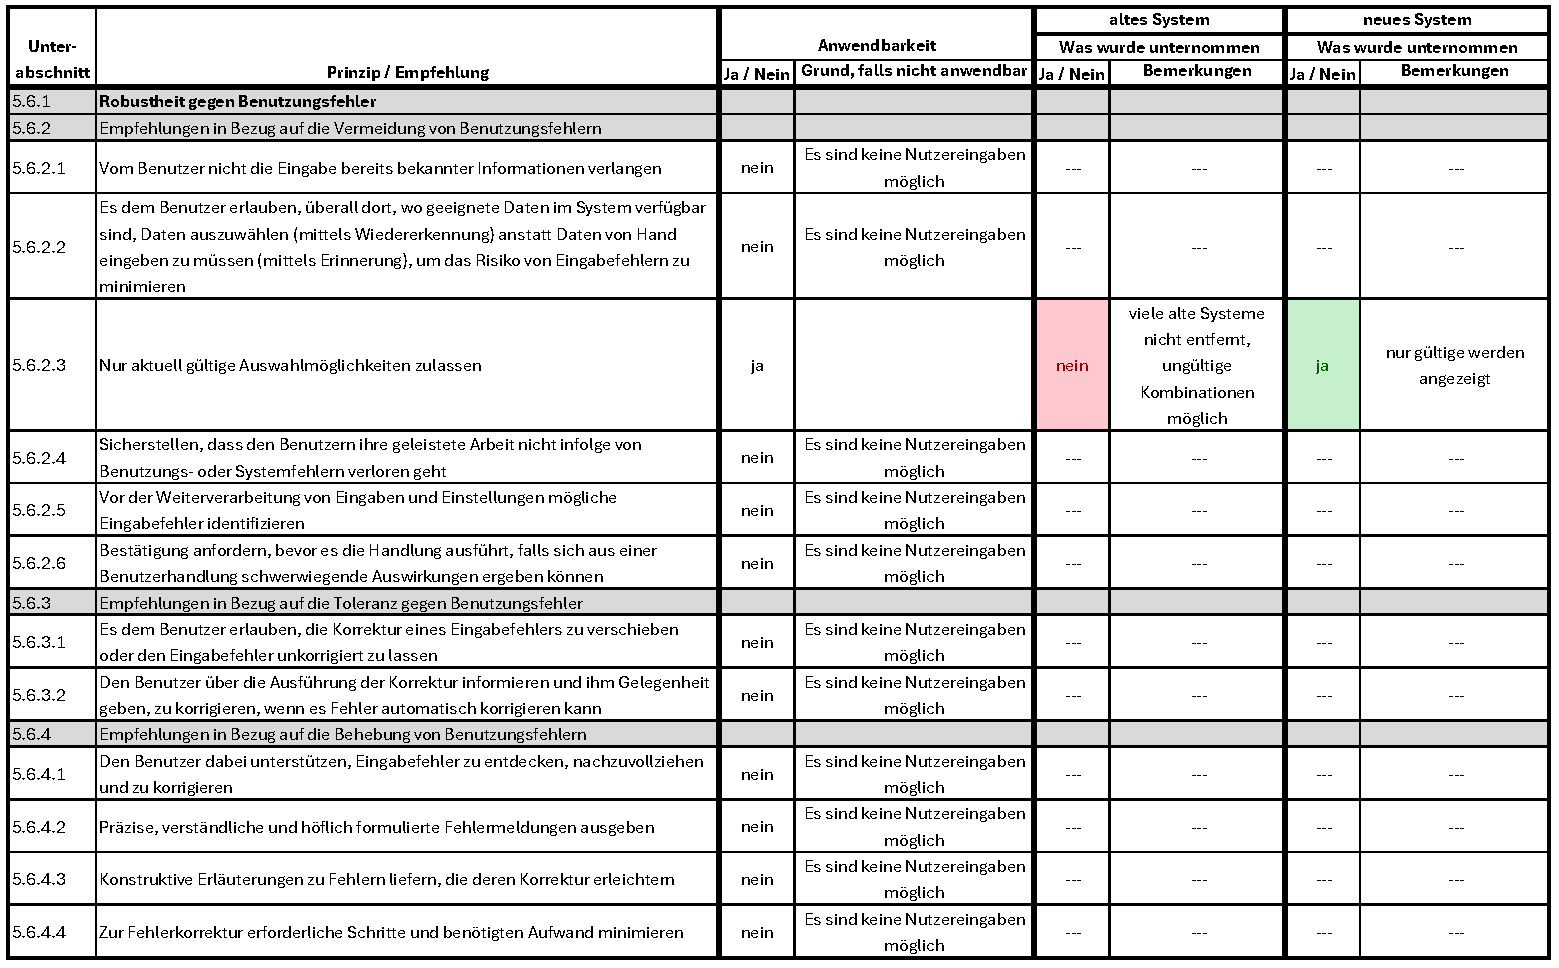
\includegraphics[width=0.95\textheight, angle=90]{Anhänge/02_ISO-Tabellen/06_Benutzungsfehler.pdf}
    \caption{Zustands- und Anforderungsanalyse sowie Vergleich des alten und neuen Systems nach \cite{DIN_EN_ISO_9241-110} (6/7 Robustheit gegen Nutzungsfehler)}
    \label{tab:Anforderungskatalog_ISO_alt_neu_6}
\end{table}

\begin{table}[H]
    \centering
    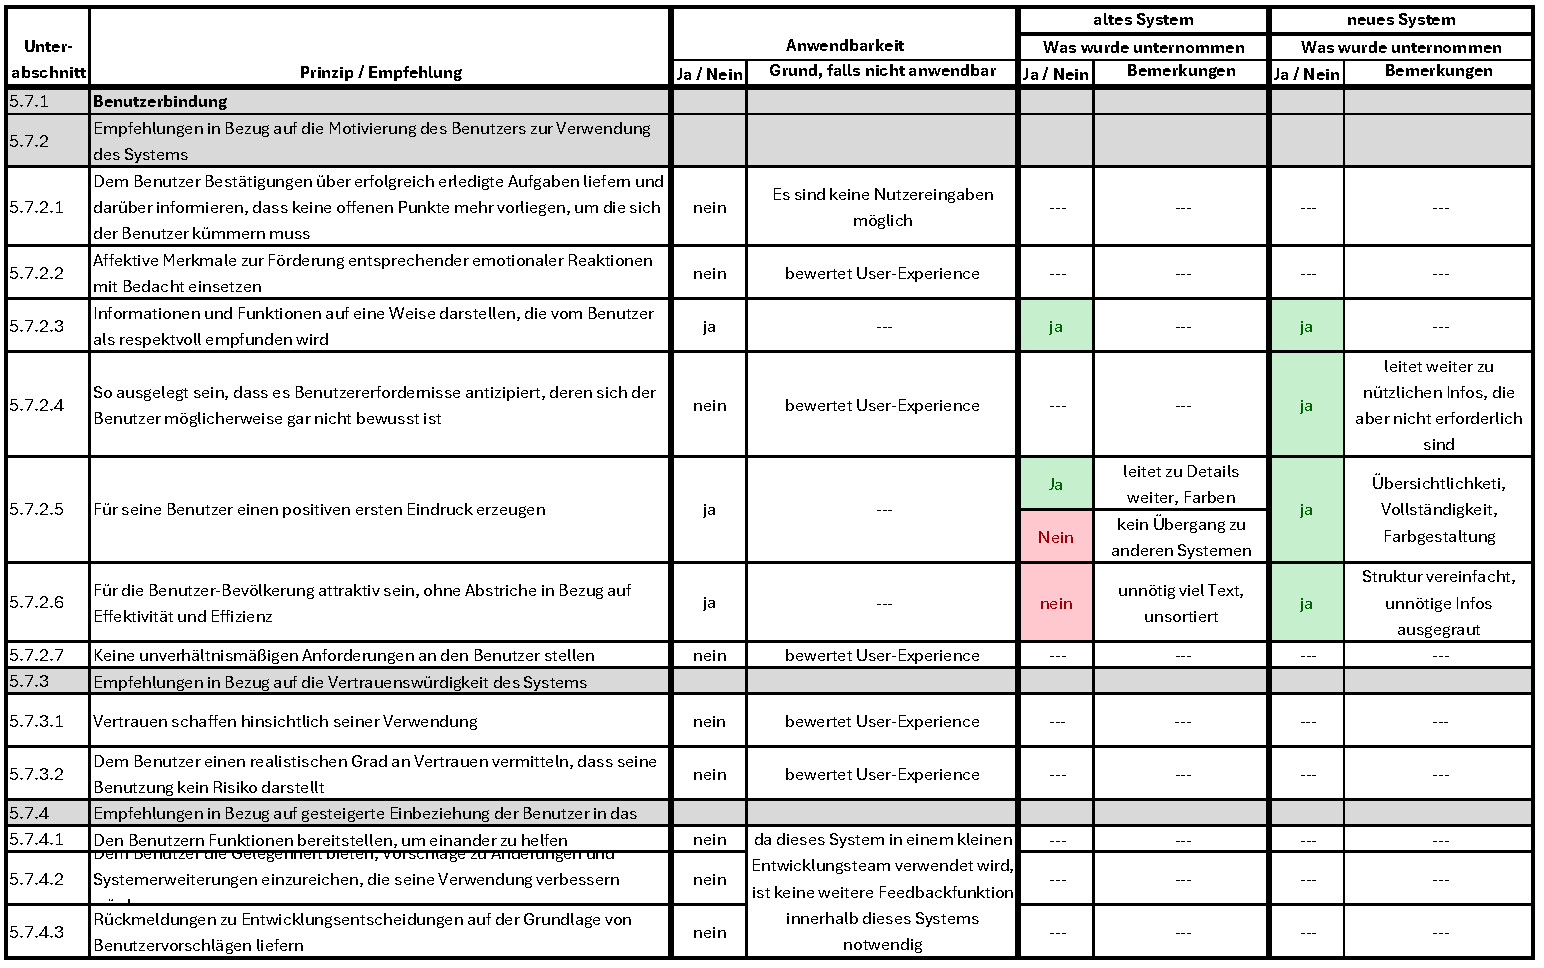
\includegraphics[width=0.95\textheight, angle=90]{Anhänge/02_ISO-Tabellen/07_Benutzerbindung.pdf}
    \caption{Zustands- und Anforderungsanalyse sowie Vergleich des alten und neuen Systems nach \cite{DIN_EN_ISO_9241-110} (7/7 Nutzerbindung)}
    \label{tab:Anforderungskatalog_ISO_alt_neu_7}
\end{table}